\documentclass[11pt, a4paper]{article}
% \usepackage[T1]{fontenc}
\usepackage[utf8]{inputenc}
\usepackage{listings}
\usepackage[margin=1.0in]{geometry}
\usepackage{color}
\usepackage{graphicx}
\usepackage{tabularx}
\usepackage{url} 

\title{Rock the net}
\author{Elias Frantar}
\author{Samuel Schmidt}
\author{Nikolaus Schrack}
\author{Gary Ye}
\date{\today{}, Wien}
\begin{document}

\lstset{ %
  backgroundcolor=\color{white},   % choose the background color; you must add \usepackage{color} or \usepackage{xcolor}
  basicstyle=\footnotesize,        % the size of the fonts that are used for the code
  breakatwhitespace=false,         % sets if automatic breaks should only happen at whitespace
  breaklines=true,                 % sets automatic line breaking
  captionpos=b,                    % sets the caption-position to bottom
% commentstyle=\color{mygreen},    % comment style
  deletekeywords={...},            % if you want to delete keywords from the given language
  escapeinside={\%*}{*)},          % if you want to add LaTeX within your code
  extendedchars=true,              % lets you use non-ASCII characters; for 8-bits encodings only, does not work with UTF-8
% frame=single,                    % adds a frame around the code
  keepspaces=true,                 % keeps spaces in text, useful for keeping indentation of code (possibly needs columns=flexible)
% keywordstyle=\color{blue},       % keyword style
% language=bash,                   % the language of the code
  morekeywords={*,...},            % if you want to add more keywords to the set
  numbers=left,                    % where to put the line-numbers; possible values are (none, left, right)
  numbersep=5pt,                   % how far the line-numbers are from the code
  numberstyle=\tiny\color{mygray}, % the style that is used for the line-numbers
  rulecolor=\color{black},         % if not set, the frame-color may be changed on line-breaks within not-black text (e.g. comments (green here))
  showspaces=false,                % show spaces everywhere adding particular underscores; it overrides 'showstringspaces'
  showstringspaces=false,          % underline spaces within strings only
  showtabs=false,                  % show tabs within strings adding particular underscores
  stepnumber=1,                    % the step between two line-numbers. If it's 1, each line will be numbered
  stringstyle=\color{mymauve},     % string literal style
  tabsize=2,                       % sets default tabsize to 2 spaces
  title=\lstname                   % show the filename of files included with \lstinputlisting; also try caption instead of title
}


\maketitle
\newpage
\tableofcontents
\newpage

\section{Task description}
% TODO
\section{Design}
% TODO
% 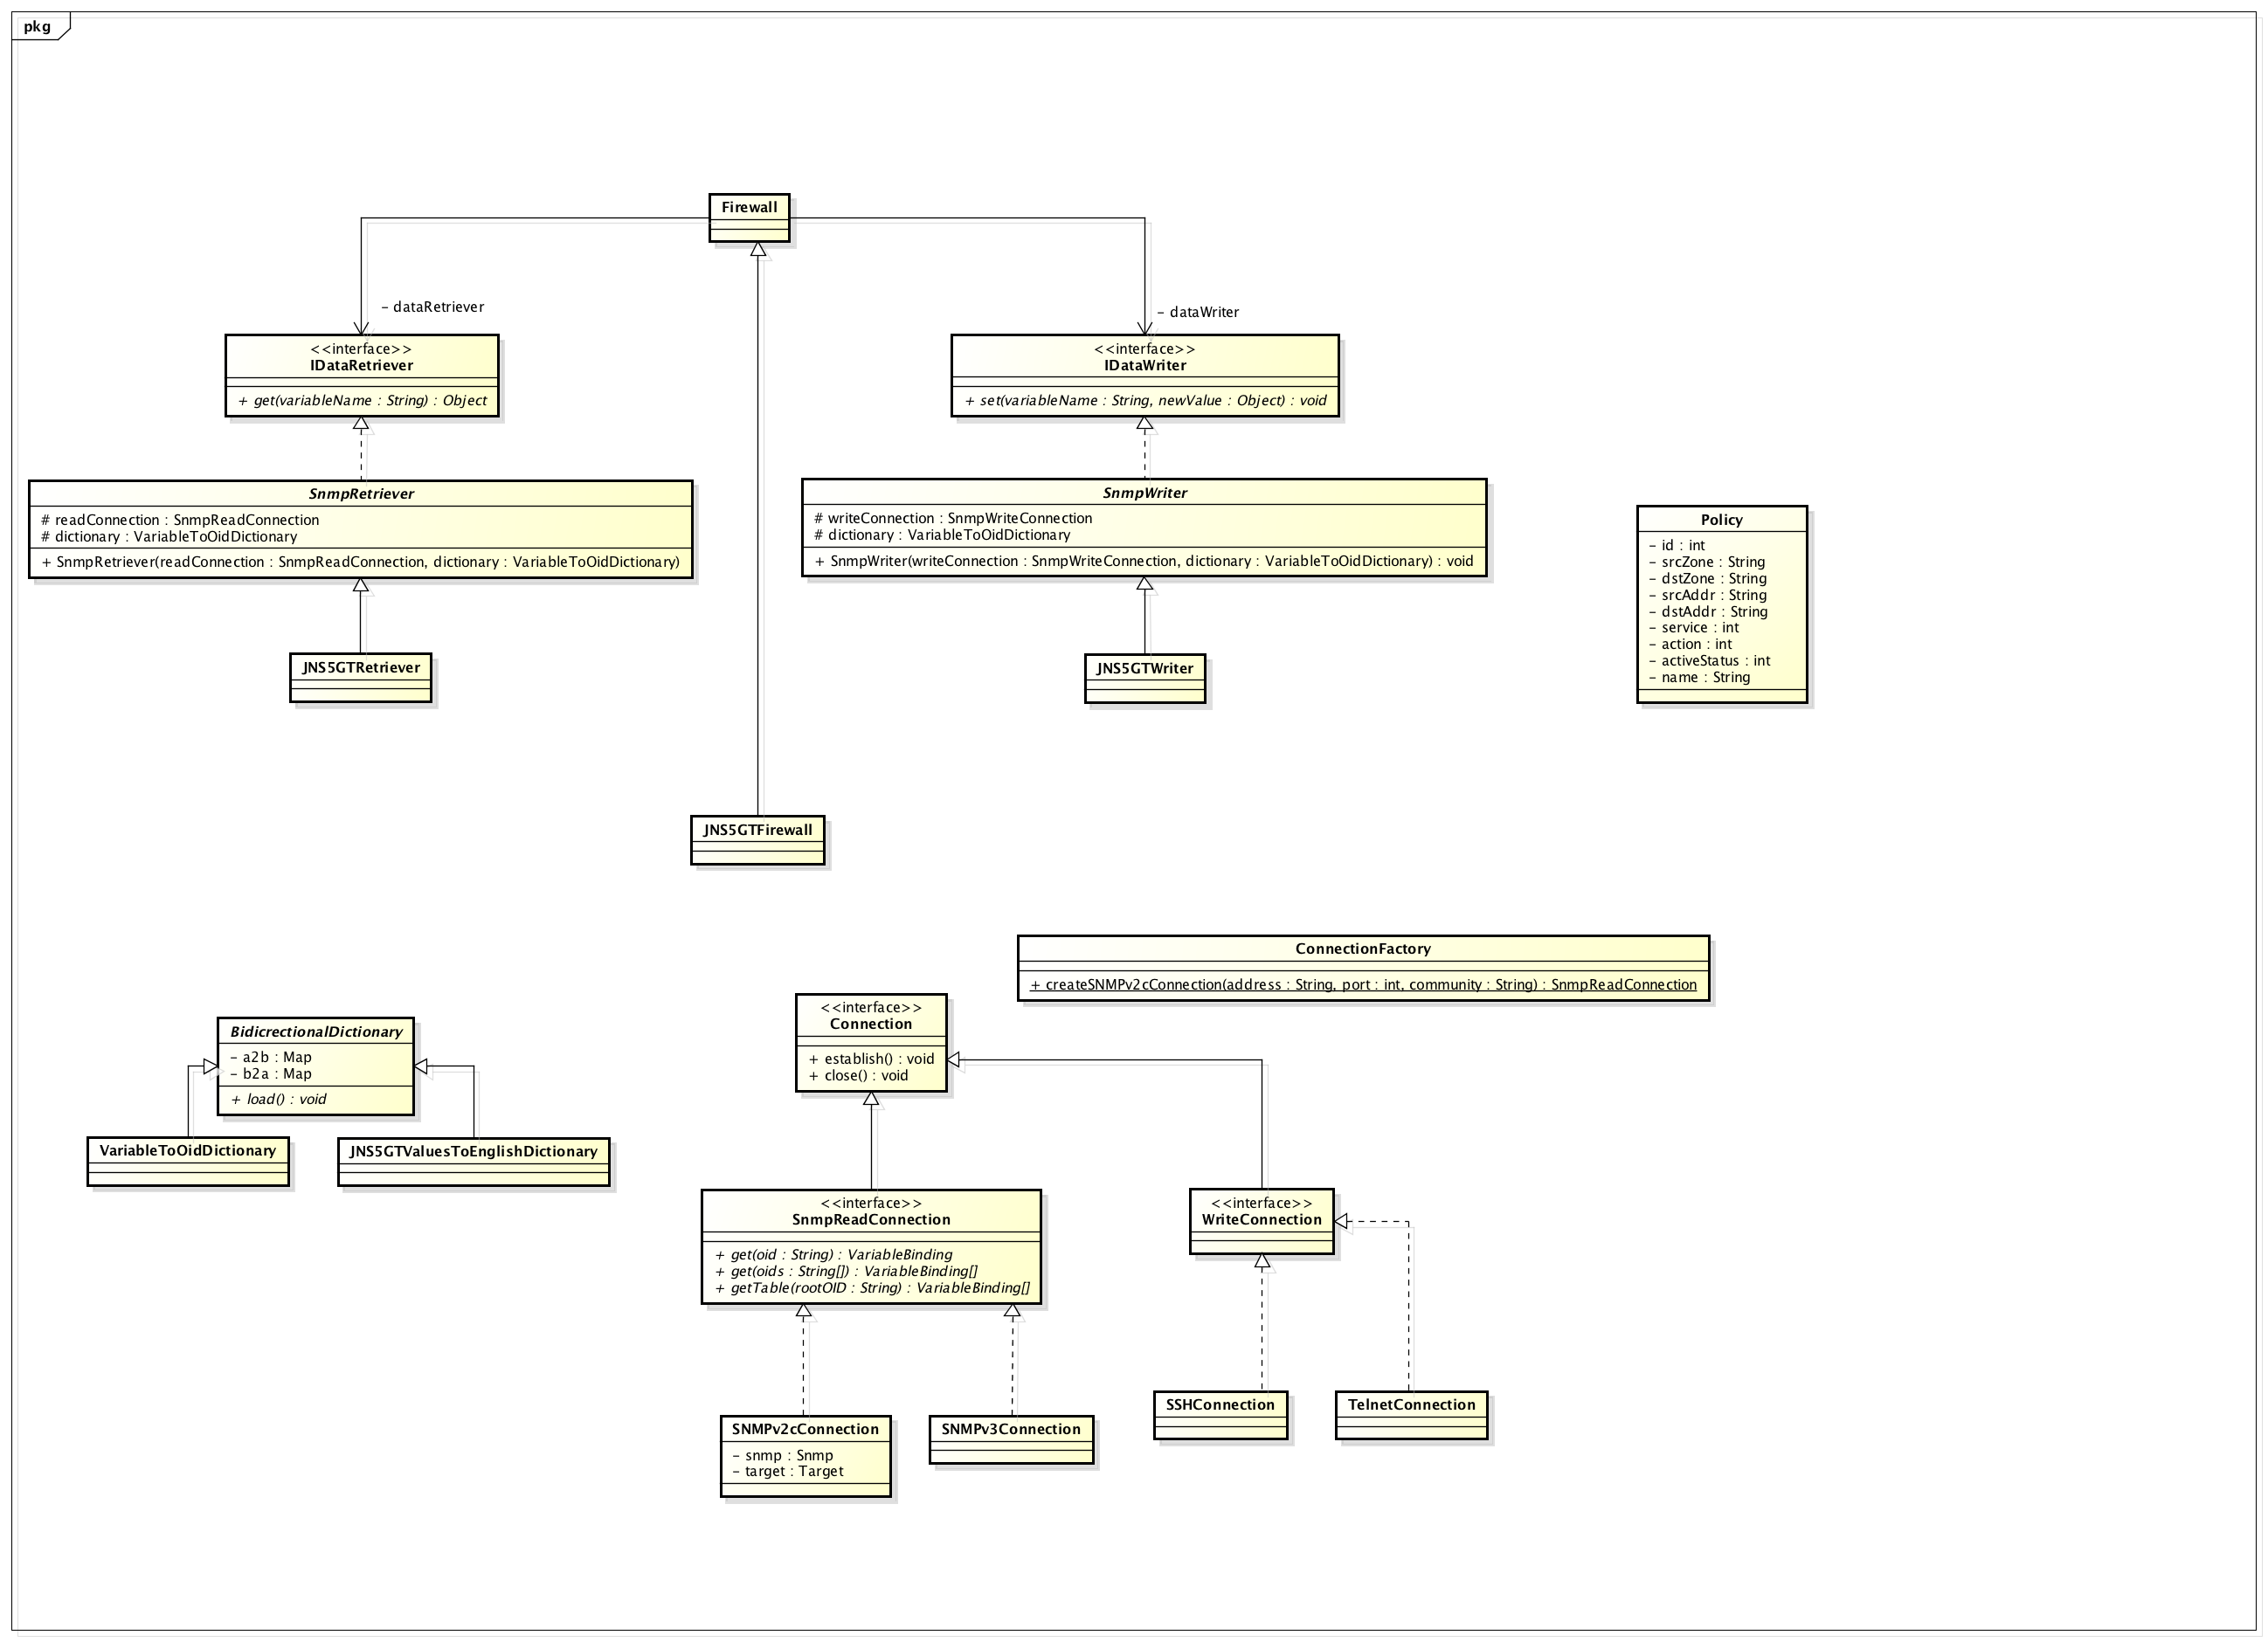
\includegraphics[width=\textwidth]{images/uml}
 
\section{Effort estimation}

\subsection{Basic Tasks}
\begin{tabular} {| l | l | l | l |} \hline
Task &	Original Estimate & Remaining Estimate & Time spent \\ \hline
Preparation for the Tasks &	20 &	0.00 & 24.50 \\ \hline
Listing firewall rules &	7 &	2 &	9.50 \\ \hline
Refreshing rules &	6 &	6 &	0.00 \\ \hline
Visualize thru put & 8 &	4 &	5.00 \\ \hline
Encapsulate the data retrieval &	4	& 0.00 &	4.00 \\ \hline
GUI	 & 10 &	7 &	8.00 \\ \hline
Final Documentation  &	8	& 2	& 5.00 \\ \hline
Basic Total	& 63 &	31.00 &	56.00 \\ \hline
\end{tabular}
\subsection{Advanced Tasks}
\begin{tabular} {| l | l | l | l |}\hline
Task &	Original Estimate & Remaining Estimate & Time spent \\ \hline
Alarm the user &	7	& 5	& 0 \\ \hline
Firewall rules CRUD &	6 &	8 & 	0 \\ \hline
Transactions by Multicast &	8 &	15 &	0 \\ \hline
Exchangeable & 5 & 0	 & 2 \\ \hline
Advanced Total & 26 &	28 &	2 \\ \hline
\end{tabular}

\subsection{Total}
\begin{description}
	\item[Original Estimate]: 89
	\item[Remaining Estimate]: 31
	\item[Time Spent]: 58
\end{description}

\section{Installation}

\section{Technologies}
\subsection{Mock-Objects}
\subsection{Java FX}
Java 8 supports Java FX, so no further installation will be needed if Java 8 is used. 

\subsubsection{Eclipse}
In Eclipse kann das Addon zum Erstellen von JavaFx Applikationen unter dem Punkt “Help” -> “Install New Software” installiert werden. Der Name ist e(fx)clipse und der Link % http://download.eclipse.org/efxclipse/updates-released/1.0.0/site. 
Jetzt kann über “New” -> “Other” -> “JavaFX Project” ein Projekt erstellt werden. 

\subsubsection{IntelliJ}
Tutorial with Java 8 and IntelliJ IDEA 13+
% http://docs.oracle.com/javase/8/scene-builder-2/work-with-java-ides/sb-with-intellij.htm 
Getting Started with JavaFX
% http://docs.oracle.com/javase/8/javafx/get-started-tutorial/jfx-overview.htm 

\subsubsection{IntelliJ - TGM Licenses}
Run IntelliJ IDEA and follow the Installation Wizard's instructions. To register for use of the software or change your existing registration details, go to Help/Register menu of the software and enter the included below the User Name and License Key(s) into the registration dialog:

User Name: TGM - Institute of Technology 
License Key: 603253-X846L-X51EC-FMQQ7-EXY9B-DO323

\subsection{Charts}
Für unsers Applikation wird ein Line Chart gebraucht, was mit JavaFX möglich ist. 
% http://docs.oracle.com/javafx/2/charts/line-chart.htm#CIHGBCFI

\subsection{SNMP - Simple Network Management Protocol}

It is, like the name says, a simple network protocol to manage and monitor the devices in a network. Practically, the monitored devices are all connected to a central system that controls them by using the “Simple Network Manager Protocol”.

Figure 1: the Router, the Server, the Switch and the Printer are connected via the SNMP to the management system.
% (Source: http://de.wikipedia.org/wiki/Simple_Network_Management_Protocol)

\subsubsection{SNMPv2c and SNMPv3 differences}

With v3 no changes to the protocol aside from added security and remote configuration enhancements (we use telnet anyway) to SNMP were added. However new textual conventions, concepts and terminology were introduced.

The core Snmp class documentation[3] offers only insight on big differences in SNMPv1(asynchronous) and v3(synchronous) implementations. TransportMapping only affects UDP/TCP/… configurations.

\subsection{MIB - Management Information Base}
As the management system wanting to read data from a device, it has to know the data of the device. The specified informations can be retrieved from the corresponding MIB. 

The MIB of the device, that is being used for this exercise, can be found here [1].

The MIB is structured like a tree (examples can be found in the Wikipedia article). Every object of the device can be identified by the OID (Object Identifier), which is just a list of numbers separated by a dot.

One can for example GET/SET the variables by using the OI of the specified object.

Also one can use a MIB browser to explore the structure [2].

[1] http://www.oidview.com/mibs/2636/JUNIPER-NSM-TRAPS.html
[2] http://ireasoning.com/mibbrowser.shtml 
[3] http://www.snmp4j.org/doc/org/snmp4j/Snmp.html 
\subsubsection{Connection}
\subsubsection{MIBs}
\subsection{Multicast-Groups}

\section{Test report}
\section{Occurred problems}
\bibliography{protokoll}{}
\bibliographystyle{plain}
\end{document}
